% Lesson 07: Including Graphics and positioning
% Link: https://www.learnlatex.org/en/more-07#storing-graphics-in-a-subdirectory
% More: Storing graphics in a subdirectory
% textwidth: takes physical paper width
% linewidth: Takes width limit set for line
\documentclass{article}
\usepackage[T1]{fontenc}
\usepackage{graphicx}

\graphicspath{{images/}{images2}}

\begin{document}
	\begin{figure}[h]
		\centering
		\includegraphics[width=0.5\textwidth]{les07_04-2.png}
		\caption{An example image}
	\end{figure}
	
	\begin{figure}[h]
		\centering
		\includegraphics[width=0.5\textwidth]{images/les07_04-2.png}
		\caption{An example image}
	\end{figure}
	\begin{figure}[h]
		\centering
		\includegraphics[width=0.5\textwidth]{les04_03-1.png}
		\caption{An example image}
	\end{figure}
	
	\begin{figure}[h]
		\centering
		\includegraphics[width=0.5\textwidth]{images2/les04_03-1.png}
		\caption{An example image}
	\end{figure}
\end{document}